\documentclass{article}
\usepackage[pdftex,
        colorlinks=true,
        urlcolor=rltblue,       % \href{...}{...} external (URL)
        filecolor=rltgreen,     % \href{...} local file
        linkcolor=rltred,       % \ref{...} and \pageref{...}
        pdftitle={Phys 20 Lab 6},
        pdfauthor={Chris Dudiak},
        pdfproducer={pdfLaTeX},
        pagebackref,
        pdfpagemode=None,
        bookmarksopen=true]{hyperref}
\usepackage{color}
\usepackage{pdfpages}
\usepackage{graphicx}
\usepackage{mathtools}
\usepackage{placeins}
\usepackage{listings}
\usepackage{verbatim}
\definecolor{rltred}{rgb}{0.75,0,0}
\definecolor{rltgreen}{rgb}{0,0.5,0}
\definecolor{rltblue}{rgb}{0,0,0.75}


\begin{document}

\title{Phys 20 Lab 6 - Root Finding}
\author{Chris Dudiak}
\date{\today}
\maketitle

\section{Part 1 - Golden Ratio Convergence of Secant Method}

Within a small distance $\epsilon$ of x, the function is approximately:
\begin{align*}
	f(x + \epsilon) = f(x) + \epsilon f'(x) + \epsilon^2 {f''(x) \over 2} + ...
\end{align*}

Evaluating at $x_1$ and $x_2$ and plugging into the step relation for the Secant Method
\begin{align*}
	f(x_3) = x_2 - f(x_2) {x_2 - x_1 \over f(x_2) - f(x_1)}
\end{align*}

we get the following:

\begin{align*}
	f(\epsilon_3) = \epsilon_2 - f(x_2) {\epsilon_2 - \epsilon_1 \over f(x_2) - f(x_1)}
\end{align*}

When a trial solution $x_i$ differs from the true root by $\epsilon$ we get:

\begin{align*}
	\epsilon_3 = \epsilon_2 - f(x_2 + \epsilon) {\epsilon_2 - \epsilon_1 \over f(x_2 + \epsilon_2) - f(x_1 + \epsilon)}
\end{align*}

Since $f(x_i)$ is zero, we get an approximation (neglecting higher order terms):
\begin{align*}
	f(x_i + \epsilon_i) \approx  \epsilon_2 f'(x_i) + \epsilon_i^2 {f''(x_i) \over 2} 
\end{align*}

Plugging this in, we get:

\begin{align*}
	\epsilon_3 \approx \epsilon_2 - (\epsilon_2 f'(x_2) + \epsilon_2^2 {f''(x_2) \over 2})  {\epsilon_2 - \epsilon \over \epsilon_2 f'(x_2) + \epsilon_2^2 
	{f''(x_2)  \over 2}  - \epsilon f'(x_1) + \epsilon^2 {f''(x_1) \over 2} }
\end{align*}

Simplifying the denominator, we find:
\begin{align*}
	f(x_2 + \epsilon_2) - f(x_1 + \epsilon) &\approx \epsilon_2 f'(x_2) + \epsilon_2^2 {f''(x_2)  \over 2}  - \epsilon f'(x_1) - \epsilon^2 {f''(x_1) \over 2} \\
	&\approx f'(x_2) * (\epsilon_2 - \epsilon) * (1 + {f''(x_2) \over 2f'(x_2)} (\epsilon_2 + \epsilon))
\end{align*}

Which gives: 

\begin{align*}
	\epsilon_3 &= \epsilon_2 - {(\epsilon_2) * (\epsilon_2  - \epsilon) * ( f'(x_2) + \epsilon_2 f''(x_2)) \over 
						f'(x_2) * (\epsilon_2 - \epsilon) * (1 + {f''(x_2) \over 2f'(x_2)} (\epsilon_2 + \epsilon))} \\
			&=  \epsilon_2 - {(\epsilon_2) * (1 + \epsilon_2 {f''(x_2) \over f'(x_2)}) \over 
						(1 + {f''(x_2) \over 2f'(x_2)} (\epsilon_2 + \epsilon))} \\
			&= {\epsilon_2 (1 + {f''(x_2) \over 2f'(x_2)} (\epsilon_2 + \epsilon)) - (\epsilon_2) (1 + \epsilon_2 {f''(x_2) \over f'(x_2)}) \over 
						(1 + {f''(x_2) \over 2f'(x_2)} (\epsilon_2 + \epsilon))} \\
			&= {\epsilon_2  \epsilon {f''(x_2) \over 2f'(x_2)}  \over 
						(1 + {f''(x_2) \over 2f'(x_2)} (\epsilon_2 + \epsilon))} \\
			&\approx \epsilon_2  \epsilon {f''(x_2) \over 2f'(x_2)}
\end{align*}

Now, assume $\epsilon_{i+1} = C \epsilon_i ^ r$ for all i where C and r are constants independent of i. Plugging this into the recurrence, we find:

\begin{align*}
	C \epsilon_2 ^ r &\approx \epsilon_2  \epsilon {f''(x_2) \over 2f'(x_2)} \\
	\epsilon_2	 ^ {r-1} &\approx \epsilon {f''(x_2) \over 2Cf'(x_2)} \\
	\epsilon_2	 &\approx \epsilon ^ {1 \over r-1} {f''(x_2) \over 2Cf'(x_2)}^ {1 \over r-1} \\
\end{align*}

So $C = {f''(x_2) \over 2Cf'(x_2)}^ {1 \over r-1}$ and $r = {1 \over r - 1}$ from the assumption. Solving for the positive r, we find the convergence rate is:

\begin{align*}
	r &= {1 \over r - 1} \\
	r^2 - r - 1&= 0 \\
	r &= {1 + \sqrt5 \over 2}
\end{align*}

Which is the Golden Ratio.

\section{Method Implementations}
The following is the code for the three method implementations:

\begin{verbatim}
def bisection(f, x1, x2):
    acc = abs(x1 - x2)
    steps = []
    x0 = (x1 + x2) / 2.0
    while acc > precision:
        x0 = (x1 + x2) / 2.0
        guess = f(x0)
        if sign(guess) == sign(f(x1)):
            x1 = x0
        else:
            x2 = x0
        acc = abs(x1 - x2)
        steps.append(guess)
    return (x0, steps)
\end{verbatim}

\begin{verbatim}
def newtonRaphson(f, fp, x1):
    guess = f(x1)
    steps = [guess]
    x2 = x1
    while abs(guess) > precision:
        x2 = x1 - guess / fp(x1)
        guess = f(x2)
        x1 = x2
        steps.append(guess)
    return (x2, steps)
\end{verbatim}

\begin{verbatim}
def secant(f, x1, x2):
    guess = f(x2)
    prev = f(x1)
    steps = [guess]
    while abs(guess) > precision:
        next = x2 - guess * (x2 - x1) / (guess - prev)
        prev = guess
        guess = f(next)
        steps.append(guess)
        x1 = x2
        x2 = next
    return (x2, steps)
\end{verbatim}

Using these methods, we plot the convergence rates of Sin(x) - .76:

\begin{figure}[h!]
	\centering
	\includegraphics[scale=.6]{"convergence"}
	\caption{Convergence Rates of the Above Methods}
\end{figure} 
\FloatBarrier

We see that the bisection method is linear, Newton is quadratic, and Secant lies in the middle at the Golden Ratio.

\section{Orbit}

Using the Newton-Raphson Method (since the derivative is easy to calculate), we get the following orbital curve:

\begin{figure}[h!]
	\centering
	\includegraphics[scale=.6]{"orbit"}
	\caption{Orbit of the Hulse-Taylor Pulsar}
\end{figure} 
\FloatBarrier

\section{Velocity Curve}

By trial and error of varying the phase, we get the following velocity curve using a $\Delta$t of .001:

\begin{figure}[h!]
	\centering
	\includegraphics[scale=.6]{"velocity"}
	\caption{Velocity Curve of the Hulse-Taylor Pulsar}
\end{figure} 
\FloatBarrier

The above graph agrees with the 1975 diagram provided using a $\phi = - {\pi \over 2}$.

\section{Orbit in Mathematica}

Using Mathematica's FindRoot function, we get the following plot for the orbit:

\begin{figure}[h!]
	\centering
	\includegraphics[scale=.6]{"orbitMath"}
	\caption{Orbit of the Hulse-Taylor Pulsar Using Mathematica}
\end{figure} 
\FloatBarrier

which agrees perfectly with the orbit found in Python using my Newton-Raphson function.

\section{Code and Info}

\subsection{Output}
The program outputs the following:
\verbatiminput{output.txt}

\subsection{Code}
Code for this week's set in Python and Appended Mathematica Code as a PDF:
\lstinputlisting[language=Python]{roots.py}

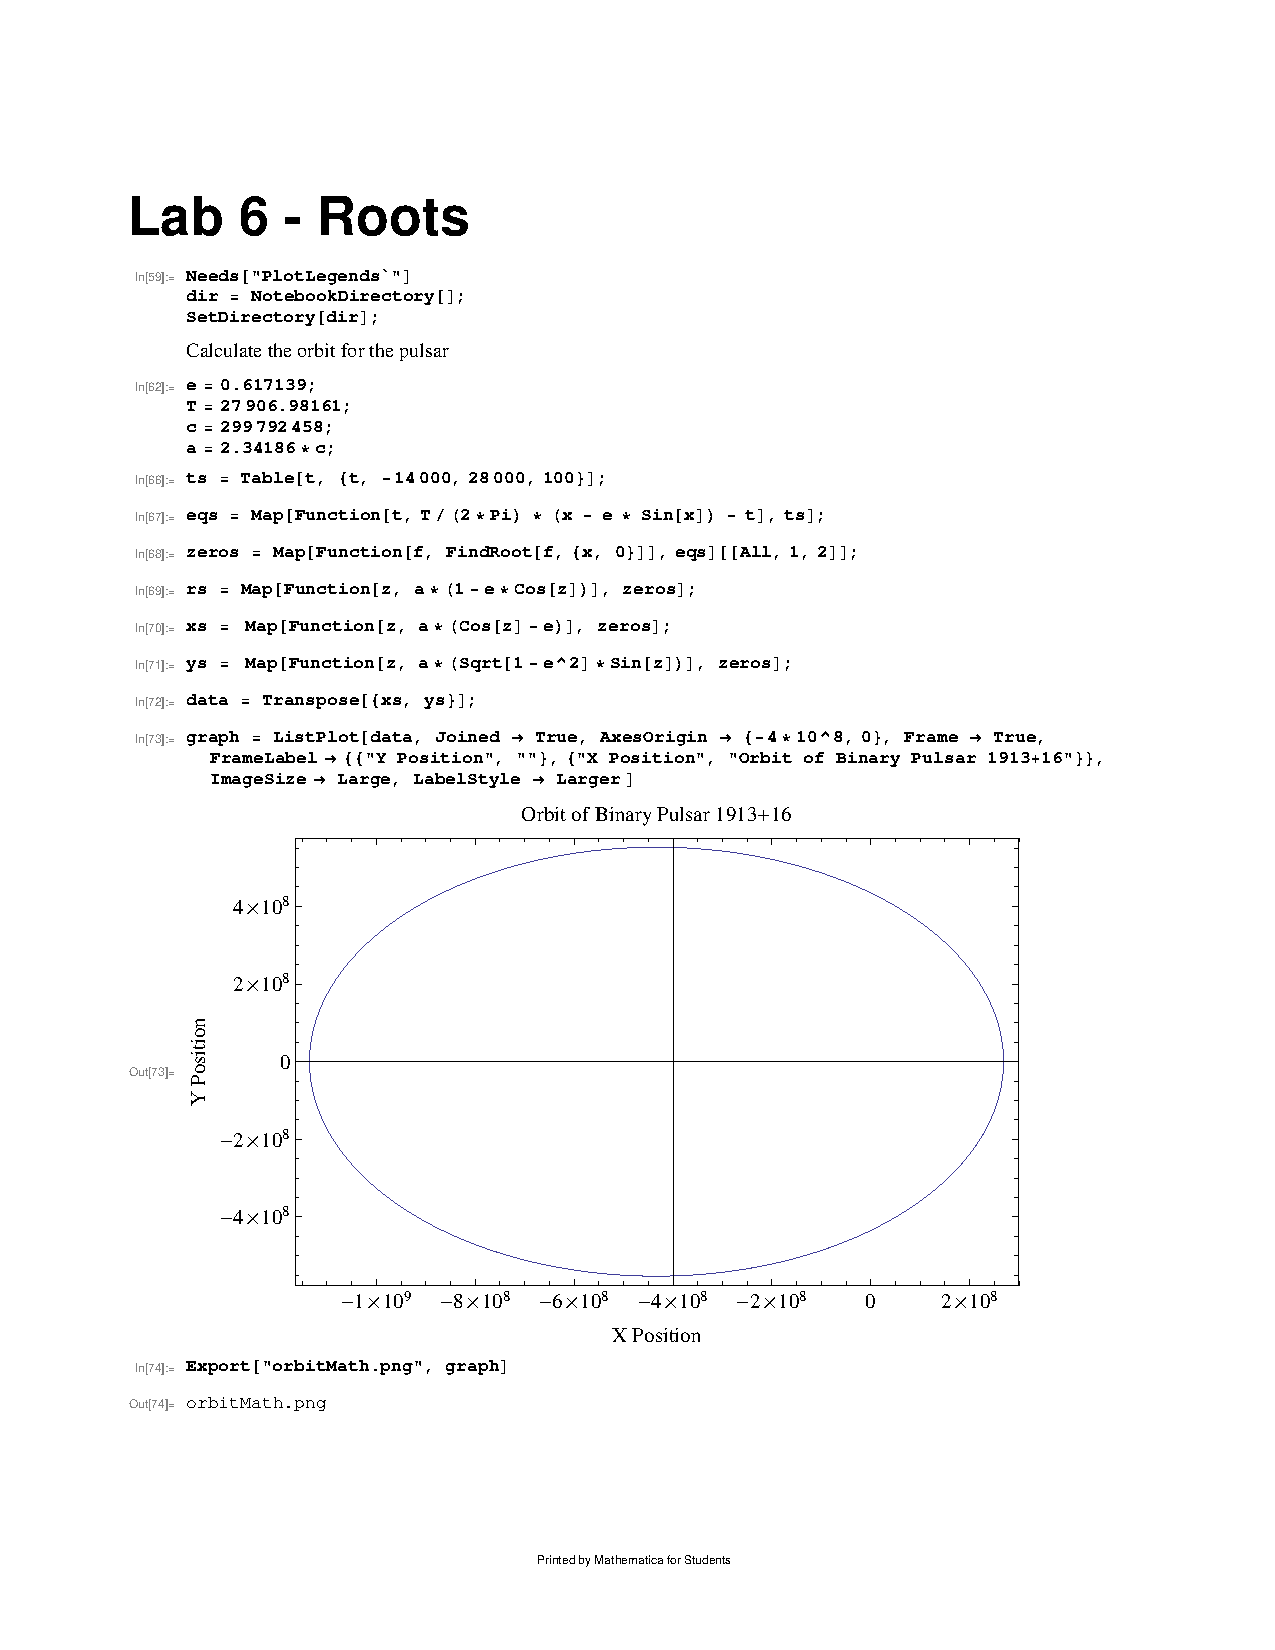
\includepdf[pages={1}]{orbitCalc.pdf}
\end{document}
